%% 
%% Copyright 2007-2020 Elsevier Ltd
%%   
%% This file is part of the 'Elsarticle Bundle'.
%% ---------------------------------------------
%%            
%% It may be distributed under the conditions of the LaTeX Project Public
%% License, either version 1.2 of this license or (at your option) any
%% later version.  The latest version of this license is in
%%    http://www.latex-project.org/lppl.txt
%% and version 1.2 or later is part of all distributions of LaTeX
%% version 1999/12/01 or later.
%% 
%% The list of all files belonging to the 'Elsarticle Bundle' is
%% given in the file `manifest.txt'.
%% 
%% Template article for Elsevier's document class `elsarticle'
%% with harvard style bibliographic references

%\documentclass[preprint,12pt,authoryear]{elsarticle}

%% Use the option review to obtain double line spacing
% \documentclass[authoryear,preprint,review,12pt]{elsarticle}

\documentclass[preprint,review,12pt]{elsarticle}

%% Use the options 1p,twocolumn; 3p; 3p,twocolumn; 5p; or 5p,twocolumn
%% for a journal layout:
%% \documentclass[final,1p,times,authoryear]{elsarticle}
%% \documentclass[final,1p,times,twocolumn,authoryear]{elsarticle}
%% \documentclass[final,3p,times,authoryear]{elsarticle}
%% \documentclass[final,3p,times,twocolumn,authoryear]{elsarticle}
%% \documentclass[final,5p,times,authoryear]{elsarticle}
%%\documentclass[final,5p,times,twocolumn,authoryear]{elsarticle}

%% For including figures, graphicx.sty has been loaded in
%% elsarticle.cls. If you prefer to use the old commands
%% please give \usepackage{epsfig}

% Document Formatting and Layout
\usepackage{geometry}
\usepackage{fancyhdr}
\usepackage{titlesec}
\usepackage{float}
\usepackage{subcaption}

% Math and Symbols
\usepackage{amsmath,amsfonts,amssymb, algorithm, algorithmic}
\usepackage{mathtools}
\usepackage{bm}
\usepackage{mathrsfs}

% Graphics and Colors
\usepackage{graphicx}
\usepackage{xcolor}
\usepackage{tikz}
\usetikzlibrary{positioning,arrows.meta}
\usepackage{pgfplots}

% Tables
\usepackage{tabularx}
\usepackage{multirow}
\usepackage{longtable}
\usepackage{colortbl}
\usepackage{booktabs}

% Lists and Enumerations
\usepackage{enumitem}

% Hyperlinks and References
\usepackage{hyperref}
% Bibliography
%\usepackage[backend=bibtex,style=numeric]{biblatex}
\usepackage{natbib}

% Miscellaneous
\usepackage{microtype}
\usepackage{siunitx}
\usepackage{todonotes}
\usepackage{lineno}

%\usepackage{todonotes}
\usepackage{caption}
\usepackage{subcaption}
\usepackage{lipsum}
\usepackage{xspace}
\usepackage{setspace}

% Command to highlight revised text
\newcommand{\rev}[1]{\textcolor{black}{#1}}
%\newcommand{\rev}[1]{\textcolor{red}{#1}}

\hyphenpenalty=10000
\exhyphenpenalty=10000
\sloppy

\journal{arXiv}
\pdfoutput=1
\pgfplotsset{compat=1.18}
\begin{document}
\linenumbers
%\modulolinenumbers[5]
\onehalfspacing

\begin{frontmatter}

%% Title, authors and addresses

%% use the tnoteref command within \title for footnotes;
%% use the tnotetext command for theassociated footnote;
%% use the fnref command within \author or \affiliation for footnotes;
%% use the fntext command for theassociated footnote;
%% use the corref command within \author for corresponding author footnotes;
%% use the cortext command for theassociated footnote;
%% use the ead command for the email address,
%% and the form \ead[url] for the home page:
%% \title{Title\tnoteref{label1}}
%% \tnotetext[label1]{}
%% \author{Name\corref{cor1}\fnref{label2}}
%% \ead{email address}
%% \ead[url]{home page}
%% \fntext[label2]{}
%% \cortext[cor1]{}
%% \affiliation{organization={},
%%            addressline={}, 
%%            city={},
%%            postcode={}, 
%%            state={},
%%            country={}}
%% \fntext[label3]{}
% \title{Fourier Neural Operators for Computing Deformation Modes in Acoustic Metamaterials with wavelet encodings of PDE parameters to toggle between deformation modes.}

%\title{Wavelet Encodings of PDE parameters Allow Fourier Neural Operators to Toggle Between Deformation Modes when Computing Deformation Fields.}

%\title{The use of wavelet encodings to allow Fourier neural operators to toggle between modes when computing deformation fields}

\title{Fourier Neural Operators using Wavelet Encodings for Solving Eigenvalue PDEs To Simulate Acoustic Metamaterial Displacement Fields}

%% use optional labels to link authors explicitly to addresses:
%% \author[label1,label2]{}
%% \affiliation[label1]{organization={},
%%             addressline={},
%%             city={},
%%             postcode={},
%%             state={},
%%             country={}}
%%
%% \affiliation[label2]{organization={},
%%             addressline={},
%%             city={},
%%             postcode={},
%%             state={},
%%             country={}}

\author[Mech]{Han Zhang}
\author[Comp]{Cynthia Rudin}
\author[Mech]{Johann Guilleminot}
\author[Mech]{L. Catherine Brinson}
\affiliation[Mech]{organization={Department of Mechanical Engineering and Materials Science, Duke University},%Department and Organization
            %addressline={}, 
            city={Durham},
            %postcode={}, 
            state={NC},
            country={USA}}
\affiliation[Comp]{organization={Department of Electrical and Computer Engineering, Duke University},%Department and Organization
            %addressline={}, 
            city={Durham},
            %postcode={}, 
            state={NC},
            country={USA}}
% \affiliation[Civil]{organization={Department of Civil and Environmental Engineering, Duke University},%Department and Organization
%             %addressline={}, 
%             city={Durham},
%             %postcode={}, 
%             state={NC},
%             country={USA}}
\begin{abstract}
%% Text of abstract
\begin{itemize}
    \item FNOs can toggle between solutions to an eigenvalue PDE with wavelet transform encodings of PDE parameters.
    \item Wavelet encodings more useful on input side than output side because the rapid oscillations do not work well with smooth loss functions.
    \item Both continuous and discontinuous geometries can be simultaneously learned by the same model. 
\end{itemize}
\end{abstract}

%%Graphical abstract
%\begin{graphicalabstract}
%\includegraphics{grabs}
%\end{graphicalabstract}

%%Research highlights
%\begin{highlights}
%\item Research highlight 1
%\item Research highlight 2
%\end{highlights}

\begin{keyword}
%% keywords here, in the form: keyword \sep keyword, up to a maximum of 6 keywords
Neural Operators \sep Metamaterials \sep Acoustics \sep Wavelet Transform \sep Machine Learning
%% PACS codes here, in the form: \PACS code \sep code

%% MSC codes here, in the form: \MSC code \sep code
%% or \MSC[2008] code \sep code (2000 is the default)

\end{keyword}

\end{frontmatter}

%\tableofcontents

%% \linenumbers

%% main text
%%%%%%%%%%%%%%%%%%%%%%%%%%%%%%%%%%%%%%%%%%%%%%%%%%%%%%%%%%%%%%%%%%%%%%
\newpage
\section{Introduction}
\label{introduction}
\begin{itemize}[noitemsep]
    \item Introduce SOTA neural operator work.
    \item Talk about the gap - eigenvalue PDEs, solution families (instead of single solution field, deterministic toggling)
    \item Talk about importance of encoding strategies for inputs generally
    \item Talk about FNO architecture specifically and why wavelet encodings are most appropriate
    \item Talk about the usefulness of FNO + wavelet encodings to simulating metamaterials (elude to, detail later in discussion)
\end{itemize}

%%%%%%%%%%%%%%%%%%%%%%%%%%%%%%%%%%%%%%%%%%%%%%%%%%%%%%%%%%%%%%%%%%%%%%
\newpage
\section{Methodology}
\label{sec:Methodology}

%%%%%%%%%%%%%%%%%%%%%%%%%%%%%%%%%%%%%%%%%%%%%%%%%%%%%%%%%%%%%%%%%%%%%%
\subsection{Metamaterial Design Space}
\label{ssec:metamaterial_design_space}
\begin{itemize}[noitemsep]
    \item Talk about choice of material A \& B.
    \item TABLE: material A \& B parameters
    \item Talk about unit cell symmetry
    \item Talk about continuous and binary subtypes and interpretation of continuous pixels
    \item FIGURE: an example continuous and binary geometry
\end{itemize}

%%%%%%%%%%%%%%%%%%%%%%%%%%%%%%%%%%%%%%%%%%%%%%%%%%%%%%%%%%%%%%%%%%%%%%
\newpage
\subsection{Wave Propagation Simulations} 
\label{ssec:wave_propagration_simulations}
\begin{itemize}[noitemsep]
    \item Talk about physics, PDE problem
    \item EQUATION - wave equation in solids - discretized PDE form
    \item Talk about IBZ discretization
    \item Talk about selection of first 6 bands
    \item Talk about inputs and outputs of FEA
    \item FIGURE: FEA data generation flowchart
\end{itemize}

\begin{figure}[H]
  \centering
  
\includegraphics[width=\textwidth]{Figures/distilled_FEA_process.png}
  \label{fig:FEA_full_process}
\end{figure}

%%%%%%%%%%%%%%%%%%%%%%%%%%%%%%%%%%%%%%%%%%%%%%%%%%%%%%%%%%%%%%%%%%%%%%
\newpage
\subsection{Dataset Construction and Downsampling} 
\label{ssec:dataset_construction}
\begin{itemize}[noitemsep]
    \item Talk about training and test dataset sizes.
    \item Talk about packaging FEA inputs and outputs into $(n \times 53\times 32 \times 32$ input tensors and $(n \times 5 \times 32 \times 32$ output tensors.
    \item OBSOLETE?: Talk about randomized downsampling to maximize geometry sampling at expense of band and wavevector sampling
    \item FIGURE: Construction of tensor inputs and outputs from FEA scalar/tensor mixed inputs and outputs.
\end{itemize}

\begin{figure}[H]
  \centering
  \begin{subfigure}[c]{0.5\textwidth}
    \centering
    
\includegraphics[scale=0.35]{Figures/distilled_input_tensorization.png}
    %
\includegraphics{Figures/distilled_input_tensorization.png}
    \caption{Construction of the input datasets}
    \label{fig:input_dataset_construction}
  \end{subfigure}%
  \hfill
  \begin{subfigure}[c]{0.5\textwidth}
    \centering
    
\includegraphics[scale=0.35]{Figures/distilled_output_tensorization2.png}
    %
\includegraphics{Figures/distilled_outout_tensorization.png}
    \caption{Construction of the output datasets}
    \label{fig:output_dataset_construction}
  \end{subfigure}
  \label{fig:dataset_construction}
\end{figure}


%%%%%%%%%%%%%%%%%%%%%%%%%%%%%%%%%%%%%%%%%%%%%%%%%%%%%%%%%%%%%%%%%%%%%%
\newpage
\subsection{Fourier Neural Operators}
\label{ssec:fourer_neural_operators}
\begin{itemize}[noitemsep]
    \item Talk about FNO purpose/motivation, high level equations
    \item Talk about FNO architecture, lifting, spectral, projection layers
    \item Talk about our FNO model's particular settings (width, height, hidden channels, layer count, nonlinear activation.)
    \item FIGURE: FNO architecture block diagram
    \item OBSOLETE?: TABLE: different FNO architectures tried
\end{itemize}

\begin{figure}[H]
  \centering
  
\includegraphics[width=\textwidth]{Figures/FNO_architecture.png}
  \label{fig:FNO_architecture}
\end{figure}

\begin{table}[H]
  \centering
  \begin{tabular}{|c|c|c|c|c|}
    \hline
    \textbf{Number of Fourier Layers} & \textbf{4} & 6 & 8 & 12 \\
    \hline
    \textbf{Number of Hidden channels} & 32 & \textbf{64} & 128 & 256 \\
    \hline
    \textbf{Non-linear Activation Function} & \textbf{GELU} & ReLU & tanh & Sigmoid \\
    \hline
  \end{tabular}
  \label{tab:FNO_hyperparameters}
\end{table}

%%%%%%%%%%%%%%%%%%%%%%%%%%%%%%%%%%%%%%%%%%%%%%%%%%%%%%%%%%%%%%%%%%%%%%
\newpage
\subsection{Wavelet Encodings}
\label{ssec:input_wavelet_encoding}
\begin{itemize}[noitemsep]
    \item Talk about naive encoding strategies for scalars for FNOs (uniform, sinusoidal)
    \item Talk about why wavelet encodings are superior for FNOs (two branches)
    \item Talk about how one would encode a single scalar, finite set (use wavelength)
    \item MOVED?: ALGORITHM: specific encoding strategy for band (moved to supplemental)
    \item Talk about how one would encode 2D scalar, finite set (add rotation)
    \item MOVED?: ALGORITHM: specific encoding strategy for wavevector (moved to supplemental)
    \item MOVED?: Talk about how one would encode a single scalar, unbounded open set (log scale, truncations)
    \item MOVED?: ALGORITHM: specific encoding strategy for eigenfrequency
    \item MOVED?: FIGURE: Eigenfrequency reconstruction loss
    \item Talk about why uniform encoding makes sense on the output side (MSE loss)
    \item OVERKILL?: FIGURE: Uniform reconstruction loss
\end{itemize}
\begin{figure}[H]
  \centering
  
\includegraphics[width=\textwidth]{Figures/eigenfrequency_encoding.png}
  \label{fig:eigenfrequency_encoding}
\end{figure}

\begin{figure}[H]
  \centering
  
\includegraphics[width=\textwidth]{Figures/eigenvalue_encode_decode_error_test.png}
  \label{fig:eigenfrequency_encoding}
\end{figure}

%%%%%%%%%%%%%%%%%%%%%%%%%%%%%%%%%%%%%%%%%%%%%%%%%%%%%%%%%%%%%%%%%%%%%%
\newpage
\subsection{Training Procedure}
\label{ssec:training_procedure}
\begin{itemize}[noitemsep]
\item Talk about loss function and optimizer choice
\item EQUATION: formal definition of loss used
\item Talk about combinations of hyperparameters tried
\item TABLE: hyperparameter combinations \todo{Move to discussion?}
\item Talk about large learning rate instability for FNOs \todo{Move to discussion?}
\end{itemize}

\begin{table}[H]
    \centering
    \begin{tabular}{|c|c|c|c|c|}
        \hline
        \textbf{Epochs} & 10 & \bm{$20$} & 50 & 100 \\ \hline
        \textbf{Learning Rate} & \bm{$10^{-4}$} & $10^{-3}$ & $10^{-2}$ & $10^{-1}$\\ \hline
        \textbf{Weight Decay} & 0 & \bm{$10^{-4}$} & $10^{-3}$ & $10^{-2}$ \\ \hline
        \textbf{Gamma} & 0 & 0.01 & \bm{$0.1$} & 0.5 \\ \hline
        \textbf{Step Size} & 0 & 1 & \bm{$4$} & 10 \\ \hline
        \textbf{Batch Size} & 64 & 128 & \bm{$256$} & 512 \\ \hline
    \end{tabular}
    \label{tab:training_hyperparameters}
\end{table}

%%%%%%%%%%%%%%%%%%%%%%%%%%%%%%%%%%%%%%%%%%%%%%%%%%%%%%%%%%%%%%%%%%%%%%
\newpage
\section{Results and Discussion}

%%%%%%%%%%%%%%%%%%%%%%%%%%%%%%%%%%%%%%%%%%%%%%%%%%%%%%%%%%%%%%%%%%%%%%
\subsection{Band and Wavevector Encoding}
\begin{itemize}[noitemsep]
\item Talk about the naive uniform field encoding approach (mode collapse)
\item FIGURE: demo of how uniform fields lead to 0 fields
\item Talk about sinusoidal encoding approach to take advantage of spectral transforms
\item FIGURE (MULTIPLE?): learning results on the sinusoidal encoding approach
\item Talk about wavelet encoding approach to take advantage of FNO dual branches
\item FIGURE (MULTIPLE?): learning results on the wavelet encoding approach
\end{itemize}

\begin{figure}[H]
    \centering
    \begin{subfigure}{\textwidth}
        \centering
        
\includegraphics[width=\textwidth]{Figures/1D sinusoidal encoding.png}
        \caption{The sinusoidal spatial encoding for band integer.}
        \label{fig:1D_sinusoidal_encoding_spatial}
    \end{subfigure}  
    \begin{subfigure}{\textwidth}
        \centering
        
\includegraphics[width=\textwidth]{Figures/1D sinusoidal encoding fft.png}
        \caption{The FFT of the above sinusoidal spatial encodings.}
        \label{fig:1D_sinusoidal_encoding_fft}
    \end{subfigure}
    \label{fig:1D_sinusoidal_encoding}
\end{figure}

\begin{figure}[H]
    \centering
    \begin{subfigure}{\textwidth}
        \centering
        
\includegraphics[width=\textwidth]{Figures/2D sinusoidal encoding.png}
        \caption{The sinusoidal spatial encoding for $x$ and $y$ wavevectors.}
        \label{fig:2D_sinusoidal_encoding_spatial}
    \end{subfigure}  
    \begin{subfigure}{\textwidth}
        \centering
        
\includegraphics[width=\textwidth]{Figures/2D sinusoidal encoding fft.png}
        \caption{The FFT of the above sinusoidal spatial encodings.}
        \label{fig:2D_sinusoidal_encoding_fft}
    \end{subfigure}
    \label{fig:2D_sinusoidal_encoding}
\end{figure}

\begin{figure}[H]
    \centering
    \begin{subfigure}{0.48\textwidth}
        \centering
        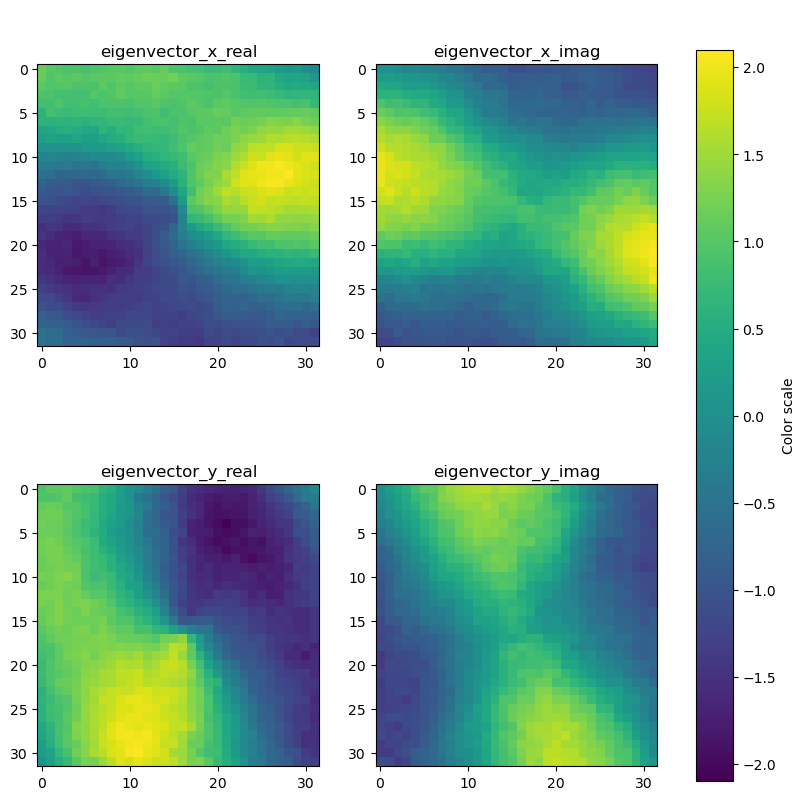
\includegraphics[width=\textwidth]{Figures/sinusoid/output_prediction3_hc64_lr1e-02_wd1e-02_ss10_gamma1e-01_e120_cropped.png}
        \caption{FNO predictions}
        \label{fig:sinusoidal_s3_prediction}
    \end{subfigure}%
    \hfill
    \begin{subfigure}{0.48\textwidth}
        \centering
        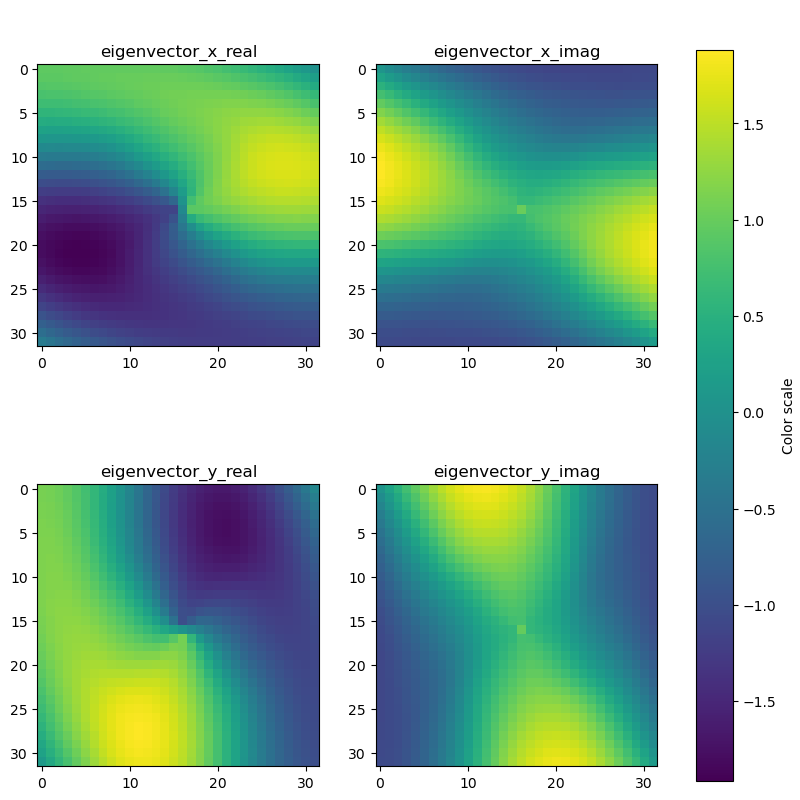
\includegraphics[width=\textwidth]{Figures/sinusoid/output_sample3_hc64_lr1e-02_wd1e-02_ss10_gamma1e-01_e120_cropped.png}
        \caption{Ground truth}
        \label{fig:sinusoidal_s3_truth}
    \end{subfigure}%
    \caption{The FNO predictions (left) and the ground truth FEA simulation (right) for a representative sample. The course structure is learned by the FNO, but the finer nuances are not grasped.}
    \label{fig:sinusoidal_s3}
\end{figure}

\begin{figure}[H]
    \centering
    \begin{subfigure}{0.48\textwidth}
        \centering
        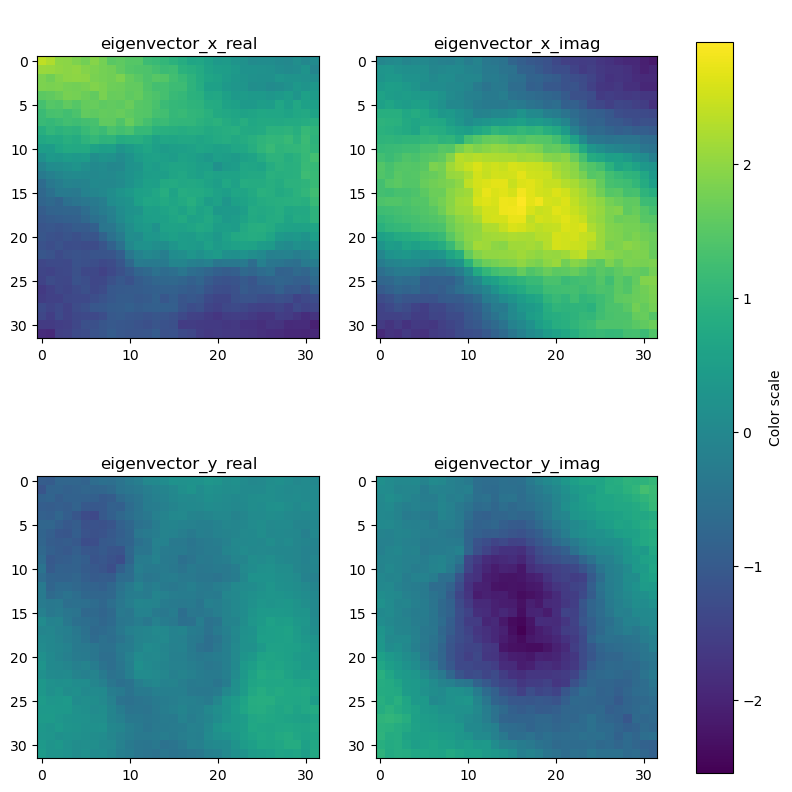
\includegraphics[width=\textwidth]{Figures/sinusoid/output_prediction5_hc64_lr1e-02_wd1e-02_ss10_gamma1e-01_e120_cropped.png}
        \caption{FNO predictions}
        \label{fig:sinusoidal_s5_prediction}
    \end{subfigure}%
    \hfill
    \begin{subfigure}{0.48\textwidth}
        \centering
        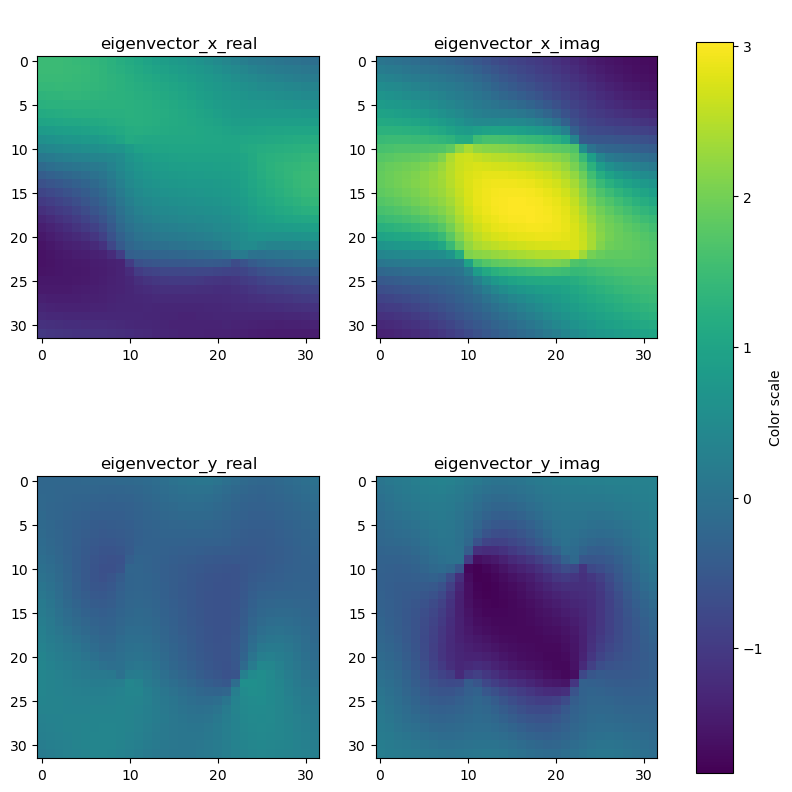
\includegraphics[width=\textwidth]{Figures/sinusoid/output_sample5_hc64_lr1e-02_wd1e-02_ss10_gamma1e-01_e120_cropped.png}
        \caption{Ground truth}
        \label{fig:sinusoidal_s5_truth}
    \end{subfigure}%
    \caption{The FNO predictions (left) and the ground truth FEA simulation (right) for another representative sample. The course structure is learned by the FNO, but the finer nuances are not grasped.}
    \label{fig:sinusoidal_s5}
\end{figure}

\begin{figure}[H]
    \centering
    \begin{subfigure}{\textwidth}
        \centering
        
\includegraphics[width=\textwidth]{Figures/1D wavelet encoding.png}
        \caption{The wavelet spatial encoding for band integer.}
        \label{fig:1D_wavelet_encoding_spatial}
    \end{subfigure}  
    \begin{subfigure}{\textwidth}
        \centering
        
\includegraphics[width=\textwidth]{Figures/1D wavelet encoding fft.png}
        \caption{The FFT of the above wavelet spatial encodings.}
        \label{fig:1D_wavelet_encoding_fft}
    \end{subfigure}
\end{figure}

\begin{figure}[H]
    \centering
    \begin{subfigure}{\textwidth}
        \centering
        
\includegraphics[width=\textwidth]{Figures/2D wavelet encoding.png}
        \caption{The wavelet spatial encoding for $x$ and $y$ wavevectors.}
        \label{fig:2D_wavelet_encoding_spatial}
    \end{subfigure}  
    \begin{subfigure}{\textwidth}
        \centering
        
\includegraphics[width=\textwidth]{Figures/2D wavelet encoding fft.png}
        \caption{The FFT of the above wavelet spatial encodings.}
        \label{fig:2D_wavelet_encoding_fft}
    \end{subfigure}
    \label{fig:2D_wavelet_encoding}
\end{figure}

\begin{figure}[H]
    \centering
    \begin{subfigure}{0.8\textwidth}
        \centering
        
\includegraphics[width=\textwidth]{Figures/input2.png}
        \caption{Random sample inputs}
        \label{fig:wavelet_s1_input}
    \end{subfigure}%
    \hfill
    \begin{subfigure}{\textwidth}
        \centering
        
\includegraphics[width=\textwidth]{Figures/output2.png}
        \caption{Random sample outputs, targets, and differences}
        \label{fig:wavelet_s1_output}
    \end{subfigure}%
    \caption{Performance of the FNO model with wavelet embedding on unencountered geometries. Inputs are shown in fig. \ref{fig:wavelet_s1_input} and outputs, targets, and differences are shown in fig. \ref{fig:wavelet_s1_output}}
    \label{fig:wavelet_s1}
\end{figure}

\begin{figure}[H]
    \centering
    \begin{subfigure}{0.8\textwidth}
        \centering
        
\includegraphics[width=\textwidth]{Figures/input4.png}
        \caption{Random sample inputs}
        \label{fig:wavelet_s2_inputs}
    \end{subfigure}%
    \hfill
    \begin{subfigure}{\textwidth}
        \centering
        
\includegraphics[width=\textwidth]{Figures/output4.png}
        \caption{Random sample outputs, targets, and differences}
        \label{fig:wavelet_s2_outputs}
    \end{subfigure}%
    \caption{Performance of the FNO model with wavelet embedding on unencountered geometries. Inputs are shown in fig. \ref{fig:wavelet_s2_input} and outputs, targets, and differences are shown in fig. \ref{fig:wavelet_s2_output}}
    \label{fig:wavelet_s2}
\end{figure}

\subsection{Hyperparameter Convergences - Output Datatype \& Batch Size}
\label{ssec:output_datatype}
\begin{itemize}[noitemsep]
% \item OBSOLETE?: Talk about training results for float64 and float16. Decision to switch to all float16.
\item OBSOLETE?: Talk about training results for batch sizes. Not much of an effect. Decision purely based on PC hardware to utilize GPU RAM. Write as a light remark on best training combination.
\item Talk about epochs to convergence.
\item FIGURE: Training and validation losses over epochs
\item Talk about high learning rate instability.
\item Talk about MSE loss that stretch different scales.
\item OBSOLETE?: Talk about trade off in sampling more geometries vs more bands/wavevectors. Too heurestic, remove.
\item Talk about mixed output vs two models approaches.
\item FIGURE (MULTIPLE?): best performing model sample outputs (consider best performance, worst performance, two randoms) (use quartiles)
\item FIGURE (MULTIPLE?): histogram of performances oversamples
\end{itemize}

\section{Conclusions}
\label{sec:Conclusion}
\begin{itemize}[noitemsep]
\item Talk about FNO capabilities in learning eigenvalue PDEs
\item Talk about importance in encoding strategy
\item Talk about continuous and binary and mixed situations
\item OBSOLETE: Talk about cautionary tales with FNOs. Focus on use, not problems since those could be overcame with other techniques.
\item Talk about scalability, generalizability, and robustness. Be careful on claims.
\item Talk about future work
\end{itemize}

\section*{Counts}
\begin{tabular}{l c}
\hline
Item & Count \\
\hline
Tables   & 2 \\
Figures  & 12+ \\
Equations& ? \\
Sections & 8\\
\hline
\end{tabular}

\section*{Declaration of Competing Interest}
The authors declare that they have no known competing financial interests or personal relationships that could have appeared to influence the work reported in this paper.

\section*{CRediT authorship contribution statement}


\section*{Data availability}
\label{sec:Repository}
The code and data in this article can be found at this GitHub repository:
\url{https://github.com/trutheresy/NO-2D-Metamaterials}.

The code for FEA computations can be found at this GitHub Repository:
\url{https://github.com/aco8ogren/2D-dispersion.git}.

\section*{Acknowledgements}

%% The Appendices part is started with the command \appendix;
%% appendix sections are then done as normal sections
%\appendix
%\section{Supplementary Figures}
%\subsection{7D Gamma \& Beta Distribution Experiment}

%\subsection{7D Gaussian Distribution Experiment}
%% \label{}

%\section{Appendix title 2}
%% \label{}

%% If you have bibdatabase file and want bibtex to generate the
%% bibitems, please use
%%
\bibliographystyle{elsarticle-num}
%\bibliographystyle{plain} 
\bibliography{references}
%%\begin{thebibliography}{00}
%% \bibitem[Author(year)]{label}
%%\end{thebibliography}

\section{Supplemental}

\subsection{Gabor Wavelet Encoding Of Dispersion Bands}
This encoding strategy is used for mapping band integers to a 2D wavelet image.
\begin{algorithm}[H]
\caption{1D Gabor Wavelet Embedding from Scalar Input}
\label{alg:1d_gabor_embedding}
\begin{algorithmic}[1]
\STATE \textbf{INPUT:} Integer \( b \); grid size \( S \leftarrow 32 \); frequency scale \( r \leftarrow 2.0 \)
\STATE Create linspace vectors \( x, y \in [-1, 1] \) with \( S \) points
\STATE Construct meshgrid \( X, Y \leftarrow \text{meshgrid}(x, y) \)
\STATE Compute base frequency:
\[
f \leftarrow (1.0 + |b|) \cdot \frac{S}{8}
\]
\STATE Compute rotation angle:
\[
\theta \leftarrow (b \bmod 8) \cdot \frac{S}{16}
\]
\STATE Rotate coordinates:
\[
X_\theta \leftarrow X \cos \theta + Y \sin \theta, \quad
Y_\theta \leftarrow -X \sin \theta + Y \cos \theta
\]
\STATE Set Gaussian envelope widths:
\[
\sigma_x \leftarrow \sigma_y \leftarrow \frac{0.3}{r}
\]
\STATE Compute Gabor wavelet embedding:
\[
\psi_b(x, y) \leftarrow
\exp\left(-\frac{X_\theta^2}{2 \sigma_x^2} - \frac{Y_\theta^2}{2 \sigma_y^2}\right)
\cdot \cos(f \cdot X_\theta)
\]
\STATE \textbf{RETURN:} \( \psi_b \in \mathbb{R}^{S \times S} \)
\end{algorithmic}
\end{algorithm}

In Algorithm \ref{alg:1d_gabor_embedding}, a grid size of 32 is used so that the image size matches that of the geometry, for ease of ingestion of the FNO model. The base frequency is set to 8, which allows for up to the first 8 bands to be encoded as unique rotations and wavelet spatial frequencies in the domain. The frequency scale $r$ and constants such as 16 and 0.3 were picked so that the images utilized most of the domain and showed sufficient scale variation across the domain.

\subsection{Gabor Wavelet Encoding of Wavevectors}
\begin{algorithm}[H]
\caption{2D Gabor Wavelet Embedding for Wavevectors}
\label{alg:2d_gabor_embedding}
\begin{algorithmic}[1]
\STATE \textbf{INPUT:} Integers \( k_x, k_y \); grid size \( S \leftarrow 32 \); frequency scale \( r \leftarrow 1.0 \)
\STATE Create linspace vectors \( x, y \in [-1, 1] \) with \( S \) points
\STATE Construct meshgrid \( X, Y \leftarrow \text{meshgrid}(x, y) \)
\STATE Compute frequencies:
\[
f_x \leftarrow (1.01 + k_x) \cdot \frac{S}{2}, \quad f_y \leftarrow (1.01 + k_y) \cdot \frac{S}{2}
\]
\STATE Compute rotation angles:
\[
\theta_x \leftarrow (k_x \bmod 5) \cdot \frac{\pi}{5}, \quad \theta_y \leftarrow (k_y \bmod 7) \cdot \frac{\pi}{7}
\]
\STATE Rotate coordinates:
\[
X_\theta \leftarrow X \cos \theta_x + Y \sin \theta_y, \quad
Y_\theta \leftarrow -X \sin \theta_x + Y \cos \theta_y
\]
\STATE Set Gaussian envelope widths:
\[
\sigma_x \leftarrow \sigma_y \leftarrow \frac{0.4}{r}
\]
\STATE Compute Gabor wavelet embedding:
\[
\psi_{k_x, k_y}(x, y) \leftarrow
\exp\left(-\frac{X_\theta^2}{2 \sigma_x^2} - \frac{Y_\theta^2}{2 \sigma_y^2}\right)
\cdot \sin(f_x X_\theta) \cdot \sin(f_y Y_\theta)
\]
\STATE \textbf{RETURN:} \( \psi_{k_x, k_y} \in \mathbb{R}^{S \times S} \)
\end{algorithmic}
\end{algorithm}

Like with Algorithm \ref{alg:1d_gabor_embedding}, in Algorithm \ref{alg:2d_gabor_embedding}, a grid size of 32 is used for FNO model ease of ingestion. The wavevectors are used to compute the base frequency and rotation angle, with different modulo numbers chosen for $x$ and $y$ to eliminate wavelet image aliasing from $x$ and $y$ being swapped. The frequency scale $r$ of 0.4 was chosen so that the images used most of the domain and showed sufficient scale variation throughout the domain.

\subsection{Gabor Wavelet Encoding of Eigenfrequencies}
Unlike with the other quantities, which are only on the input side and always known, this quantity is on the output side, and must be computed, then interpreted. Thus, in addition to an encoding strategy for model ease of learning, we also need a decoding compliment, to transform the model friendly format back to a simple numeric quantity - the frequency response of the material $\omega$ at that spatial wave input.
\begin{algorithm}[H]
\caption{Eigenfrequency Wavelet Encoding}
\label{alg:eigenfrequency_wavelet_encoding}
\begin{algorithmic}[1]
\STATE \textbf{INPUT:} Eigenfrequency \( s>0 \); image size \( S \leftarrow 32 \); frequency bounds \( [s_{\min}, s_{\max}] \); spectral-index bounds \( [k_{\min}, k_{\max}] \)
\STATE Set constants \( \gamma \leftarrow 1,\ \phi \leftarrow 0,\ \sigma \leftarrow 8,\ \theta_{\min}\leftarrow \pi/30,\ \theta_{\max}\leftarrow \pi/2-\pi/30 \)
\STATE Compute log-domain values:
\[
\ell_s \leftarrow \log s,\quad \ell_{\min}\leftarrow \log s_{\min},\quad \ell_{\max}\leftarrow \log s_{\max}
\]
\STATE Compute normalized position and spectral index:
\[
t \leftarrow \mathrm{clip}\!\left(\frac{\ell_s-\ell_{\min}}{\ell_{\max}-\ell_{\min}},0,1\right),\quad
k \leftarrow k_{\min} + t\,(k_{\max}-k_{\min})
\]
\STATE Compute log width per unit \(k\):
\[
\Delta_\ell \leftarrow \frac{\ell_{\max}-\ell_{\min}}{k_{\max}-k_{\min}}
\]
\STATE Compute orientation from within-band log position:
\[
\theta \leftarrow \theta_{\min} + \left(\frac{(\ell_s-\ell_{\min})\bmod \Delta_\ell}{\Delta_\ell}\right)\left(\theta_{\max}-\theta_{\min}\right)
\]
\STATE Build centered grid \(X,Y \in \{-S/2,\dots,S/2-1\}\), then rotate:
\[
X_\theta \leftarrow X\cos\theta + Y\sin\theta,\quad
Y_\theta \leftarrow -X\sin\theta + Y\cos\theta
\]
\STATE Set envelope widths \( \sigma_x \leftarrow \sigma,\ \sigma_y \leftarrow \gamma \sigma_x \), and carrier frequency \( \omega \leftarrow 2\pi k/S \)
\STATE Compute wavelet image:
\[
\psi_s \leftarrow
\exp\!\left(-\frac{1}{2}\left(\frac{X_\theta^2}{\sigma_x^2}+\frac{Y_\theta^2}{\sigma_y^2}\right)\right)\cos(\omega X_\theta+\phi)
\]
\STATE \textbf{RETURN:} \( \psi_s \in \mathbb{R}^{S\times S},\ k,\ \theta \)
\end{algorithmic}
\end{algorithm}

\begin{algorithm}[H]
\caption{Eigenfrequency Wavelet Decoding}
\label{alg:eigenfrequency_wavelet_decoding}
\begin{algorithmic}[1]
\STATE \textbf{INPUT:} Wavelet image \( \psi \in \mathbb{R}^{S\times S} \); bounds \( [s_{\min}, s_{\max}] \), \( [k_{\min}, k_{\max}] \), \( [\theta_{\min}, \theta_{\max}] \)
\STATE Set constants for centroid refinement: radius \(R\leftarrow 3\), power \(p\leftarrow 2\)
\STATE Mean-center image \( \psi_c \leftarrow \psi - \mathrm{mean}(\psi) \), then compute the centered 2D discrete Fourier magnitude:
\[
\hat{\psi}(k_x,k_y)\leftarrow \sum_{m=0}^{S-1}\sum_{n=0}^{S-1}\psi_c(m,n)\,
\exp\!\left(-2\pi i\!\left(\frac{k_x m}{S}+\frac{k_y n}{S}\right)\right),\quad
F(k_x,k_y)\leftarrow |\hat{\psi}(k_x,k_y)|
\]
\STATE Keep upper-half-plane spectral support (plus positive-frequency center row) and find dominant peak index \( (r^{*},c^{*}) \)
\STATE Define symmetric peak partner about center, then compute weighted local centroid around \( (r^{*},c^{*}) \) within radius \(R\), using weights \(w=F^p\) and excluding points closer to the symmetric partner
\STATE Convert refined centroid to wavevector coordinates \( (k_x,k_y) \), then:
\[
k_{\mathrm{ext}} \leftarrow \sqrt{k_x^2+k_y^2},\quad
\theta_{\mathrm{ext}} \leftarrow \operatorname{atan2}(k_y,k_x)\bmod \pi
\]
\STATE Map extracted \(k\) to approximate log-frequency:
\[
\ell_{\mathrm{approx}} \leftarrow \ell_{\min} + \mathrm{clip}\!\left(\frac{k_{\mathrm{ext}}-k_{\min}}{k_{\max}-k_{\min}},0,1\right)\,(\ell_{\max}-\ell_{\min})
\]
\STATE Let \( \Delta_\ell \leftarrow (\ell_{\max}-\ell_{\min})/(k_{\max}-k_{\min}) \), compute within-band position from angle:
\[
\alpha \leftarrow \mathrm{clip}\!\left(\frac{\theta_{\mathrm{ext}}-\theta_{\min}}{\theta_{\max}-\theta_{\min}},0,1\right),\quad
\delta_\ell \leftarrow \alpha\,\Delta_\ell
\]
\STATE Find nearest consistent log-frequency by testing neighboring bands \(b-1,b,b+1\):
\[
\ell^\star \leftarrow \arg\min_{\ell \in \{\ell_{\min} + j\Delta_\ell + \delta_\ell\}} |\ell-\ell_{\mathrm{approx}}|
\]
\STATE Clip \( \ell^\star \) to \( [\ell_{\min},\ell_{\max}] \), then decode:
\[
s_{\mathrm{ext}} \leftarrow \exp(\ell^\star)
\]
\STATE \textbf{RETURN:} \( s_{\mathrm{ext}},\ k_{\mathrm{ext}},\ \theta_{\mathrm{ext}} \)
\end{algorithmic}
\end{algorithm}

Algorithms \ref{alg:eigenfrequency_wavelet_encoding} and \ref{alg:eigenfrequency_wavelet_decoding} summarize the forward and inverse mapping used for eigenfrequency wavelet images. The forward mapping places eigenfrequency on a log scale and jointly encodes magnitude and orientation into a Gabor-like pattern. The inverse mapping recovers an estimate by spectral peak detection with centroid refinement, followed by a consistency step that combines extracted magnitude and angle to reconstruct the most likely log-frequency.


\end{document}

\endinput
%%
%% End of file `elsarticle-template-harv.tex'.
